\documentclass[14pt]{extarticle}
\usepackage[english,ukrainian]{babel}
\usepackage[utf8]{inputenc}
\usepackage[T1]{fontenc}

\usepackage{amsmath,amssymb}
\usepackage{parskip}
\usepackage{graphicx}
\usepackage{xcolor}
\usepackage{tcolorbox}
\tcbuselibrary{skins}
\usepackage[framemethod=tikz]{mdframed}
\usepackage{chngcntr}
\usepackage{enumitem}
\usepackage{hyperref}
\usepackage{float}
\usepackage{subfig}
\usepackage{esint}
\usepackage[top=2.5cm, left=3cm, right=3cm, bottom=4.0cm]{geometry}
\usepackage[table]{xcolor}
\usepackage{algorithm}
\usepackage{algpseudocode}
\usepackage{listings}

\title{Домашня робота з курсу ``Теоретична механіка''}
\author{Студента 3 курсу групи МП-31 Захарова Дмитра}
\date{\today}

\begin{document}

\maketitle

\section*{Завдання 48.13}

\textbf{Умова.} Див. рис. \ref{fig:1}.
\begin{figure}[H]
    \centering
    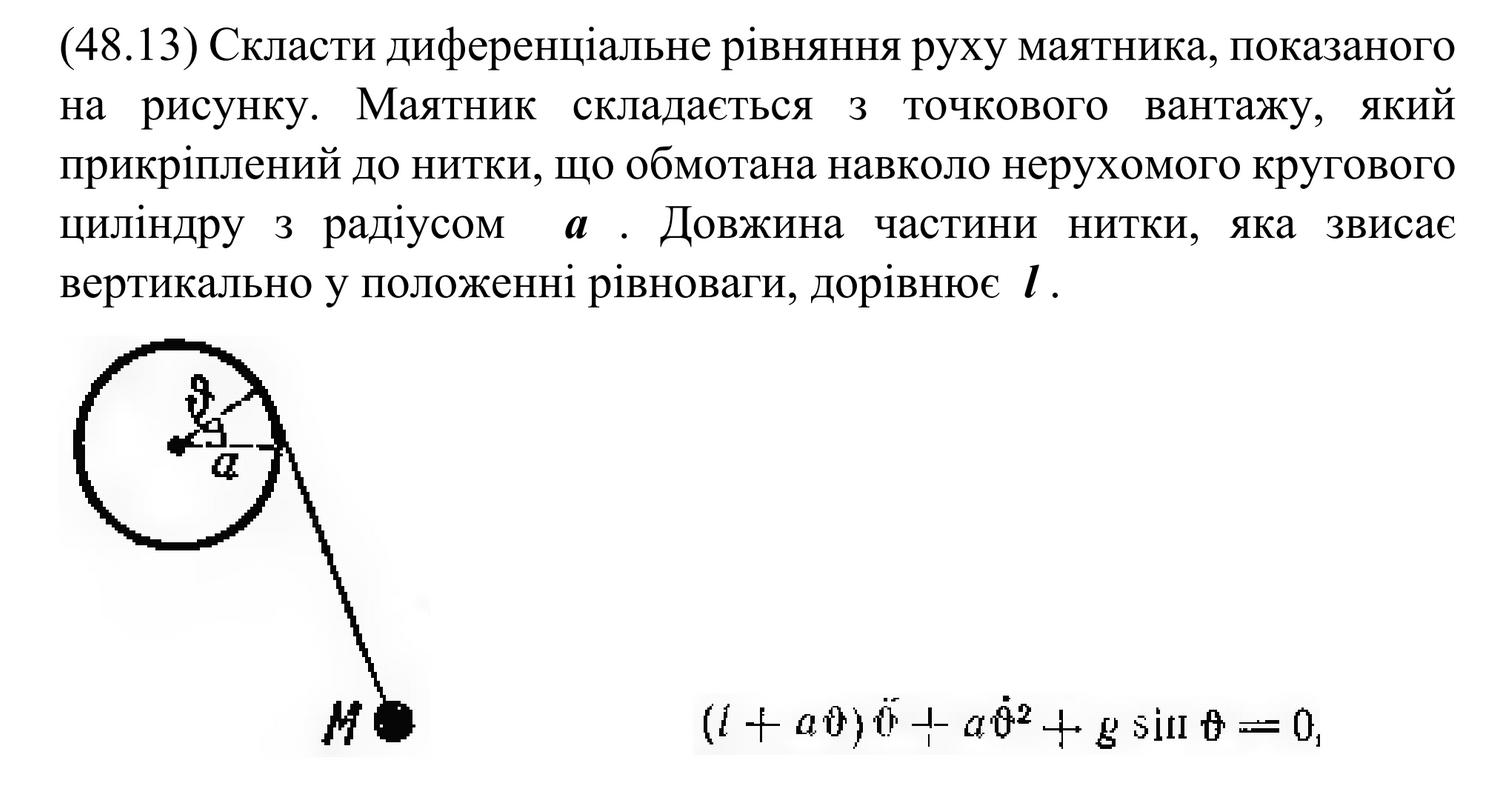
\includegraphics[width=\textwidth]{images/hw_14/fig_1.png}
    \caption{Умова до завдання}
    \label{fig:1}
\end{figure}

\textbf{Розв'язок.} Запишемо Лагранжиан нашої системи, вважаючи кут $\theta$ від вертикалі праворуч головною координатою. 

Швидкість кульки дорівнює $(\ell-\theta a)\dot{\theta}$ (оскільки довжина частини, що висить, дорівнює $\ell-\theta a$, котру ми далі множиму на кутову швидкість $\dot{\theta}$). 

Тепер розберемося з потенціальною енергією. За нульовий рівень обираємо положення рівноваги. Коли ми відвели шарик на кут $\theta$, то довжина частини, що залишилась, стала $\ell - \theta a$. Також ця величина множиться на $\cos\theta$, щоб знайти саме проекцію на висоту. Плюс до цього, точка відвіса зрушилася на $a\theta$ по колу, а в проекції на $a\sin\theta$ Таким чином, потенціальна енергія:
\begin{gather*}
V(\theta) = mg(a\sin\theta+(\ell-\theta a)\cos\theta) - mg\ell  \\
= mg\left[a(\sin\theta - \theta \cos\theta) + \ell(\cos\theta-1)\right]
\end{gather*}

Отже, маємо наступний Лагранжиан:
\[
\mathcal{L}(\theta,\dot{\theta}) = T(\theta,\dot{\theta}) - V(\theta) = \frac{m(\ell-\theta a)^2\dot{\theta}^2}{2} - mg\left[(\ell-\theta a)\cos\theta + a\sin\theta - \ell\right]
\]
Запишемо рівняння Лагранжа:
\[
\frac{d}{dt}\left(\frac{\partial\mathcal{L}}{\partial\dot{\theta}}\right) - \frac{\partial \mathcal{L}}{\partial\theta} = 0
\]
Отже, знаходимо похідні:
\[
\frac{\partial\mathcal{L}}{\partial\dot{\theta}} = \frac{\partial T(\theta,\dot{\theta})}{\partial \dot{\theta}} = m(\ell-\theta a)^2\dot{\theta} \implies \frac{d}{dt}\left(\frac{\partial\mathcal{L}}{\partial\dot{\theta}}\right) = m(\ell-\theta a)^2\ddot{\theta}-2ma\dot{\theta}^2(\ell-\theta a)
\]
\[
\frac{\partial \mathcal{L}}{\partial\theta} = -ma\dot{\theta}^2(\ell-\theta a) - mga\cos\theta + mg\sin\theta(\ell-\theta a) + mga\cos\theta
\]
Якщо спростити:
\[
\frac{d}{dt}\left(\frac{\partial\mathcal{L}}{\partial\dot{\theta}}\right) = m(\ell-\theta a)\left[(\ell-\theta a)\ddot{\theta}-2a\dot{\theta}^2\right], \; \frac{\partial\mathcal{L}}{\partial\theta} = m(\ell-\theta a)(g\sin\theta - a\dot{\theta}^2)
\]
Оскільки $\frac{d}{dt}\left(\frac{\partial\mathcal{L}}{\partial\dot{\theta}}\right)=\frac{\partial\mathcal{L}}{\partial\theta}$, то отримуємо
\[
(\ell-\theta a)\ddot{\theta} - 2a\dot{\theta}^2 = g\sin\theta - a\dot{\theta}^2 \implies \boxed{(\ell-\theta a)\ddot{\theta} - a\dot{\theta}^2 - g\sin\theta = 0}
\]

\pagebreak
\section*{Завдання 18.6}

\textbf{Розв'язок.} Праву частину рівняння ми з вами вивели. Виведемо ліву.

Нехай $\varphi$ -- це кут, на який повернувся коток 1. Тоді його кінетичну енергію можна записати як $T_1=\frac{I_1\dot{\varphi}^2}{2} = \frac{m_1R_1^2\dot{\varphi}^2}{4}$. Потенціальна енергія з часом не змінюється, тому вираз для неї записувати не будемо.

Лінійна швидкість руху мотузки в точці дотику з першим катком $R_1\dot{\varphi}$. Вона така сама для другого катка, тому кутова швидкість другого катка $\dot{\psi} = \frac{R_1\dot{\varphi}}{2R_2}$. У нього вже як кінетична, так і потенціальна енергії змінюються. 

Кінетична енергія, на відміну від першого катку, складається з обертальної та поступальної компонент, тобто
\[
T_2=\frac{m_2v_2^2}{2}+\frac{I_2\dot{\psi}^2}{2} = \frac{m_2}{2}\left(\frac{R_1\dot{\varphi}}{2}\right)^2 + \frac{m_2R_2^2}{4} \cdot \left(\frac{R_1\dot{\varphi}}{2R_2}\right)^2 = \frac{3m_2R_1^2\dot{\varphi}^2}{16}
\]
Потенціальна ж енергія змінилася на $m_2g\Delta h$. Для зміни висоти помітимо, що каток пройшов відстань $\psi R_2$, а отже зміна висоти $\Delta h = \psi R_2 \sin\alpha=\frac{R_1\varphi}{2R_2} \cdot R_2\sin\alpha=\frac{R_1\varphi\sin\alpha}{2}$. Отже, загальний Лагранжиан системи:
\[
\mathcal{L}(\varphi,\dot{\varphi}) = T_1+T_2-V_2 = \frac{m_1R_1^2\dot{\varphi}^2}{4} + \frac{3m_2R_2^2\dot{\varphi}^2}{16} - \frac{m_2gR_1\varphi\sin\alpha}{2}
\]
Записуємо рівняння Лагранжа:
\[
\frac{d}{dt}\left(\frac{\partial\mathcal{L}}{\partial\dot{\varphi}}\right) - \frac{\partial \mathcal{L}}{\partial\varphi} = M
\]
Знаходимо похідні:
\[
\frac{\partial\mathcal{L}}{\partial\dot{\varphi}} = \frac{m_1R_1^2\dot{\varphi}}{2} + \frac{3m_2R_1^2\dot{\varphi}}{8} \implies \frac{d}{dt}\left(\frac{\partial\mathcal{L}}{\partial\dot{\varphi}}\right) = \frac{m_1R_1^2\ddot{\varphi}}{2} + \frac{3m_2R_1^2\ddot{\varphi}}{8}
\]
\[
\frac{\partial\mathcal{L}}{\partial\varphi} = -\frac{m_2gR_1\sin\alpha}{2}
\]
Таким чином:
\[
\frac{m_1R_1^2\ddot{\varphi}}{2} + \frac{3m_2R_1^2\ddot{\varphi}}{8} + \frac{m_2gR_1\sin\alpha}{2} = M
\]

\end{document}

